\documentclass[12pt,titlepage]{article}
\usepackage[margin=1.25in]{geometry}
\usepackage{graphicx,amsmath,blindtext,minted}

%% Variables definition
\newcommand{\vSubject}{Basic Programming Practicum}
\newcommand{\vSubtitle}{Function 1}
\newcommand{\vName}{Dicha Zelianivan Arkana}
\newcommand{\vNIM}{2241720002}
\newcommand{\vClass}{1i}
\newcommand{\vDepartment}{Information Technology}
\newcommand{\vStudyProgram}{D4 Informatics Engineering}

%% [START] Tikz related stuff
\usepackage{tikz}
\usetikzlibrary{svg.path,calc,shapes.geometric,shapes.misc}
\tikzstyle{terminator} = [rectangle, draw, text centered, rounded corners = 1em, minimum height=2em]
\tikzstyle{preparation} = [chamfered rectangle, chamfered rectangle sep=0.75em, draw, text centered, minimum height = 2em]
\tikzstyle{process} = [rectangle, draw, text centered, minimum height=2em]
\tikzstyle{decision} = [diamond, aspect=2, draw, text centered, minimum height=2em]
\tikzstyle{data}=[trapezium, draw, text centered, trapezium left angle=60, trapezium right angle=120, minimum height=2em]
\tikzstyle{connector} = [line width=0.25mm,->]
%% [END] Tikz related stuff

%% [START] Fancy header related stuff
\usepackage{fancyhdr}
\pagestyle{fancy}
\setlength{\headheight}{15pt} % compensate fancyhdr style
\fancyhead{}
\fancyfoot{}
\fancyfoot[L]{\thepage}
\fancyfoot[R]{\textit{\vSubject - \vSubtitle}}
\renewcommand{\footrulewidth}{0.4pt}% default is 0pt, overline for footer
%% [END] Fancy header related stuff

%% [START] Custom tabular command related stuff
\usepackage{tabularx}
\newcommand{\details}[2]{
    #1 & #2  \\
}
%% [END] Custom tabular command related stuff

%% [START] Figure related stuff
\newcommand{\image}[3][1]{
    \begin{figure}[h]
        \centering
        \includegraphics[#1]{#2}
        \caption{#3}
        \label{#3}
    \end{figure}
}
%% [END] Figure related stuff

\begin{document}
\begin{titlepage}
    \centering
    \vfill
    {\bfseries\LARGE
        \vSubject\\
        \vskip0.25cm
        \vSubtitle
    }
    \vfill
    
\includegraphics[width=6cm]{images/polinema-logo.png}
    \vfill
    {
        \textbf{Name}\\
        \vName\\
        \vskip0.5cm
        \textbf{NIM}\\
        \vNIM\\
        \vskip0.5cm
        \textbf{Class}\\
        \vClass\\
        \vskip0.5cm
        \textbf{Department}\\
        \vDepartment\\
        \vskip0.5cm
        \textbf{Study Program}\\
        \vStudyProgram
    }
\end{titlepage}

\tableofcontents

\pagebreak

\section{Laboratory}
\subsection{Experiment 1}
\begin{enumerate}
    \item Create a new project
    \item Create a new class, name it \texttt{Greeting}
    \item {
        Create a function called \texttt{giveGreeting} inside the class

        \begin{minted}[autogobble,fontsize=\small]{java}
            public class Greeting {
                static void giveGreeting() {
                    System.out.println("Hello! Good morning");
                }
            }
        \end{minted}
    }
    \item {
        Create a \texttt{main} function inside the class, and execute the \texttt{giveGreeting}
        function from within the \texttt{main} function.

        \begin{minted}[autogobble,fontsize=\small]{java}
            public class Greeting {
                static void giveGreeting() {
                    System.out.println("Hello! Good morning");
                }

                public static void main(String[] args) {
                    giveGreeting();
                }
            }
        \end{minted}
    }
    \pagebreak
    \item {
        Compile and run the program

        \begin{figure}[h]
            \centering
            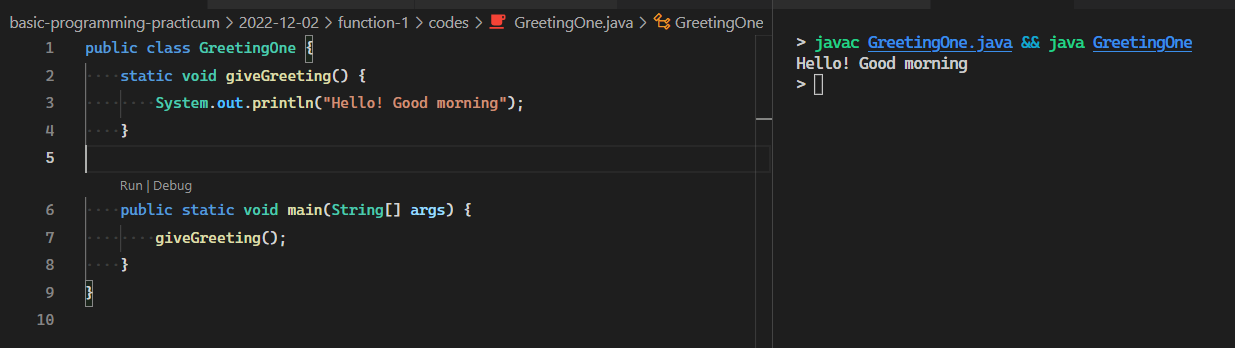
\includegraphics[width=.8\textwidth]{./images/greeting-one.png}
            \caption{Experiment 1 code and output}
        \end{figure}
    }
\end{enumerate}

\subsection{Experiment 2}
\begin{enumerate}
    \item {
        Using the class that was created in Experiment 1, add function called\\
        \texttt{saySomething} inside the \texttt{Greeting} class

        \begin{minted}[autogobble,fontsize=\small]{java}
            public class Greeting {
                static void giveGreeting() {
                    System.out.println("Hello! Good morning");
                }

                static void saySomething(String expression) {
                    System.out.println(expression);
                }

                public static void main(String[] args) {
                    giveGreeting();
                }
            }
        \end{minted}
    }
    \item {
        Execute the \texttt{saySomething} function from inside the \texttt{main} function

        \begin{minted}[autogobble,fontsize=\small]{java}
            public class Greeting {
                static void giveGreeting() {
                    System.out.println("Hello! Good morning");
                }

                static void saySomething(String expression) {
                    System.out.println(expression);
                }

                public static void main(String[] args) {
                    giveGreeting();
                    String exp = "Welcome to Java Programming";
                    saySomething(exp);
                }
            }
        \end{minted}
    }
    \item {
        Compile and run the program

        \begin{figure}[h]
            \centering
            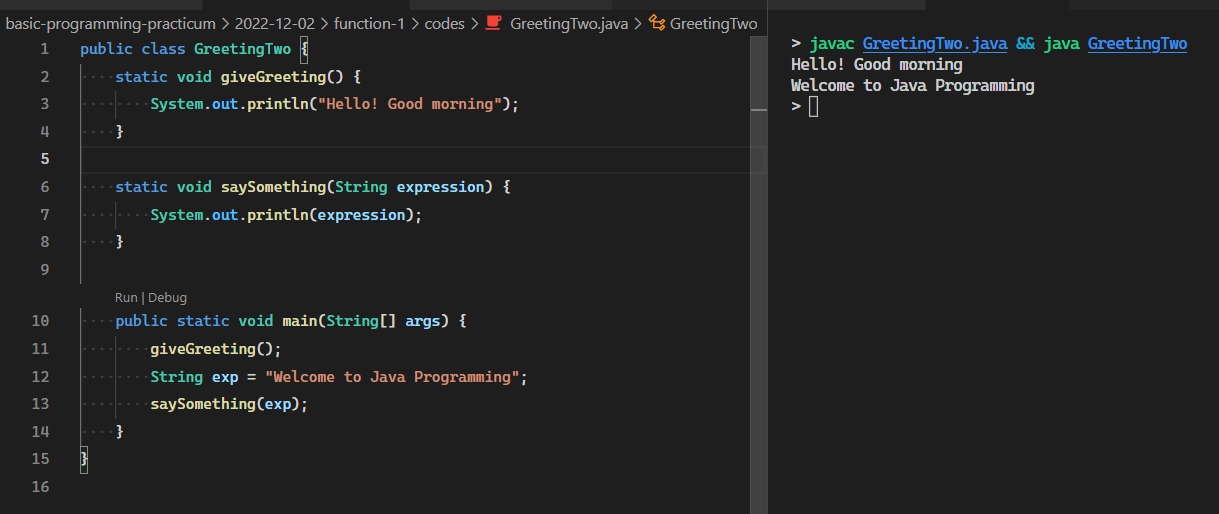
\includegraphics[width=.8\textwidth]{./images/greeting-two.png}
            \caption{Experiment 2 code and output}
        \end{figure}
    }
\end{enumerate}

\subsection{Experiment 3}
\begin{enumerate}
    \item Create a new class, name it \texttt{Square}
    \item {
        Create a function named \texttt{squareArea} inside that class which returns the value
        \texttt{area} (int), with the input parameter \texttt{side} (int)

        \begin{minted}[autogobble,fontsize=\small]{java}
            public class Square {
                static int squareArea(int side) {
                    int area = side * side;
                    return area;
                }
            }
        \end{minted}
    }
    \item {
        Create a \texttt{main} function inside the class, and execute the \texttt{squareArea}
        function from within the \texttt{main} function.

        \begin{minted}[autogobble,fontsize=\small]{java}
            public class Square {
                static int squareArea(int side) {
                    int area = side * side;
                    return area;
                }

                public static void main(String[] args) {
                    int a = squareArea(5);
                    System.out.println("Area of a square with side = 5 is " + a);
                }
            }
        \end{minted}
    }
    \item {
        Compile and run the program

        \begin{figure}[h]
            \centering
            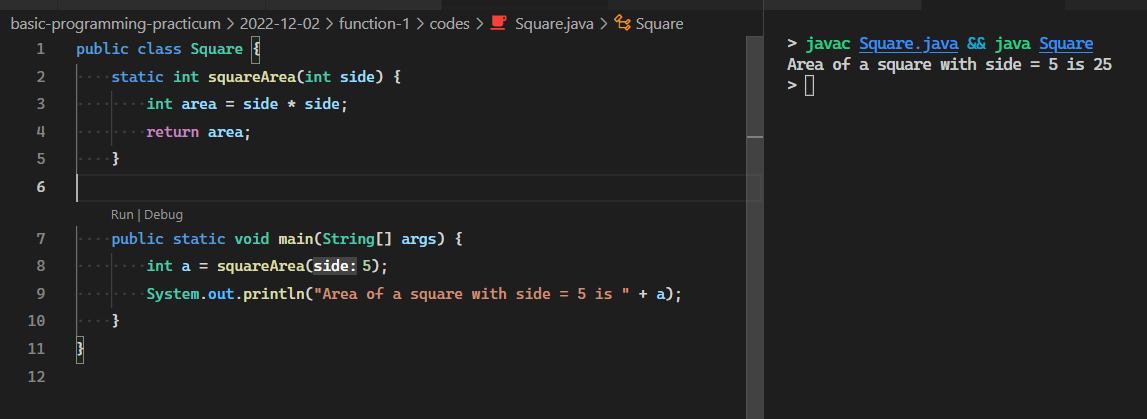
\includegraphics[width=.8\textwidth]{./images/square.png}
            \caption{Experiment 3 code and output}
        \end{figure}
    }
\end{enumerate}

\subsection{Experiment 4}
\begin{enumerate}
    \item Create a new class, name it \texttt{ArithmeticOperation}
    \item {
        Create a function named \texttt{multiplication} inside that class which returns the 
        value \texttt{H} (int) and input parameters \texttt{C} and \texttt{D} (int)

        \begin{minted}[autogobble,fontsize=\small]{java}
            public class ArithmeticOperation {
                static int multiplication(int C, int D) {
                    int H;
                    H = (C + 10) % (D + 19);
                    return H;
                }
            }
        \end{minted}
    }
    \item {
        Create a function called \texttt{substraction} inside that class which returns the value
        \texttt{X} (int) and input parameters \texttt{A} and \texttt{B} (int) and calls the
        \texttt{multiplication} function.

        \begin{minted}[autogobble,fontsize=\small]{java}
            public class ArithmeticOperaion {
                static int multiplication(int C, int D) {
                    int H;
                    H = (C + 10) % (D + 19);
                    return H;
                }

                static int substraction(int A, int B) {
                    int X;
                    A = A + 7;
                    B = B + 4;
                    X = multiplication(A, B);
                    return X;
                }
            }
        \end{minted}
    }
    \item {
        Create a \texttt{main} function inside the class, and execute the substraction function from
        within the \texttt{main} function. Don't forget to add the \texttt{Scanner} library.

        \begin{minted}[autogobble,fontsize=\small]{java}
            public static void main(String[] args) {
                int value1, value2;
                Scanner input = new Scanner(System.in);
                System.out.print("Input value 1: ");
                value1 = input.nextInt();
                System.out.print("Input value 2: ");
                value2 = input.nextInt();
                int result = substraction(value1, value2);
                System.out.println("The result is " + result);
            }
        \end{minted}
    }
    \item {
        Compile and run the program.

        \begin{figure}[h]
            \centering
            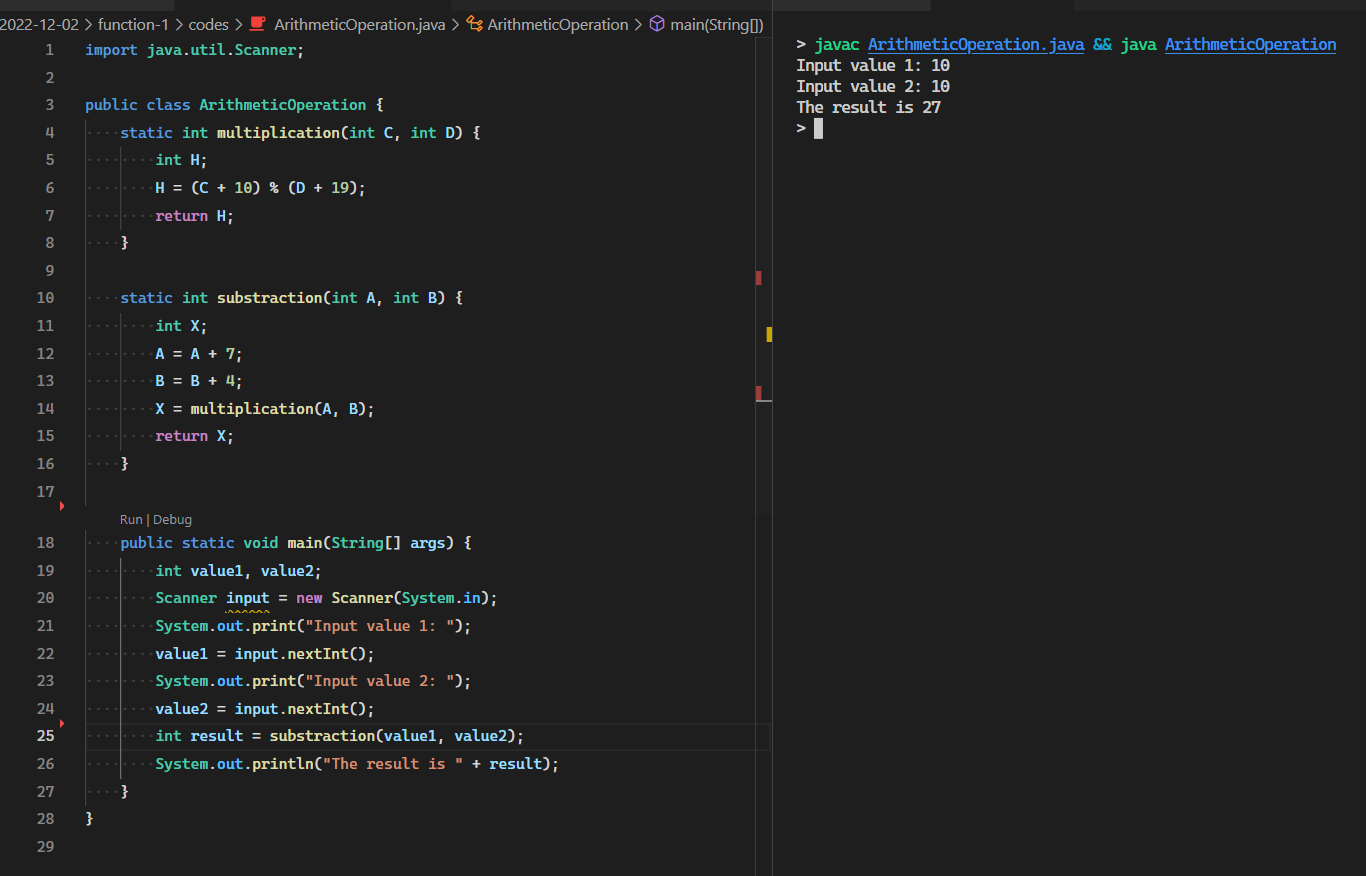
\includegraphics[width=.75\textwidth]{./images/arithmetic-operation.png}
            \caption{Experiment 4 code and output}
        \end{figure}
    }
\end{enumerate}

\subsection{Experiment 5}
\begin{enumerate}
    \item Create a new class, name it \texttt{MultiParameter}
    \item {
        Create a function called \texttt{Print} (void) inside the class using two types of
        parameter data, namely \texttt{String} and \texttt{int}

        \begin{minted}[autogobble,fontsize=\small]{java}
            public class MultiParameter {
                static void Print(String str, int... a) {
                    System.out.println("String: " + str);
                    System.out.println("Number of parameters: " + a.length);
                    for (int i : a) {
                        System.out.print(i + " ");
                    }
                    System.out.println("");
                }
            }
        \end{minted}
    }
    \item {
        Create a \texttt{main} function inside the class, and execute the \texttt{Print} function
        from within the \texttt{main} function.

        \begin{minted}[autogobble,fontsize=\small]{java}
            public static void main(String[] args) {
                Print("Basic Programming", 85, 90);
                Print("Information Technology", 1, 2, 3, 4, 5);
                Print("Politeknik Negeri Malang");
            }
        \end{minted}
    }
    \item {
        Compile and run the program

        \begin{figure}[h]
            \centering
            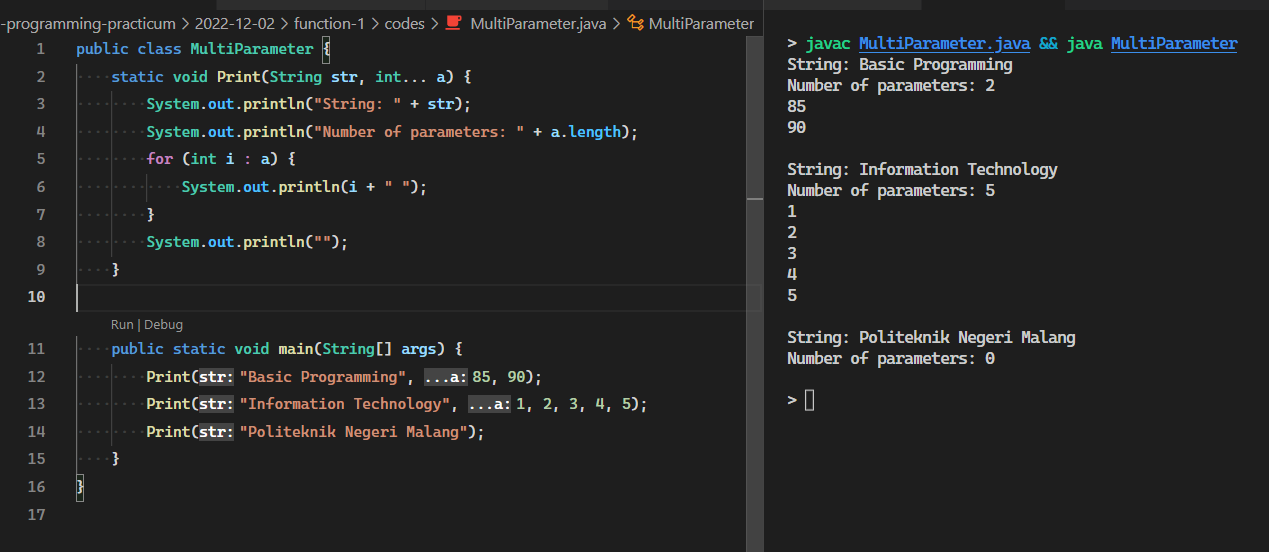
\includegraphics[width=.8\textwidth]{./images/multi-parameter.png}
            \caption{Experiment 5 code and output}
        \end{figure}
    }
\end{enumerate}

\subsection{Experiment 6}
\begin{enumerate}
    \item Create a new class, name it \texttt{Geometry1}
    \item {
        Create a program to calculate the area of a rectangle and volume of blocks wihtout using functions

        \begin{minted}[autogobble,fontsize=\small]{java}
            public static void main(String[] args) {
                Scanner input = new Scanner(System.in);
                int length, width, height, area, volume;
                System.out.print("Enter a length value: ");
                length = input.nextInt();
                System.out.print("Enter a width value: ");
                width = input.nextInt();
                System.out.print("Enter a height value: ");
                height = input.nextInt();
                area = length * width;
                System.out.println("Area of rectangle is " + area);
                volume = length * width * height;
                System.out.println("Volume of block is " + volume);
            }
        \end{minted}
    }
    \item Create another new class, name it \texttt{Geomety2}
    \item {
        \texttt{Geometry2} contains the program code for calculating the area of a rectangle
        and the volume of a block by using a function, so that there are three functions,
        namely \texttt{calculateArea}, \texttt{calculateVolume}, and the \texttt{main} function.

        \begin{itemize}
            \item {
                \texttt{calculateArea} function
                \begin{minted}[autogobble,fontsize=\small]{java}
                    static int calculateArea(int lgt, int wdt) {
                        int a = lgt * wdt;
                        return a;
                    }
                \end{minted}
            }
            \item {
                \texttt{calculateVolume} function
                \begin{minted}[autogobble,fontsize=\small]{java}
                    static int calculateVolume(int hgt, int a, int b) {
                        int vol = calculateArea(a, b) * hgt;
                        return vol;
                    }
                \end{minted}
            }
            \item {
                \texttt{main} function
                \begin{minted}[autogobble,fontsize=\small]{java}
                    public static void main(String[] args) {
                        Scanner input = new Scanner(System.in);
                        int length, width, height, area, volume;
                        System.out.print("Enter a length value: ");
                        length = input.nextInt();
                        System.out.print("Enter a width value: ");
                        width = input.nextInt();
                        System.out.print("Enter a height value: ");
                        height = input.nextInt();
                        area = calculateArea(length, width);
                        System.out.println("Area of rectangle is " + area);
                        volume = calculateVolume(height, length, width);
                        System.out.println("Volume of block is " + volume);
                    }
                \end{minted}
            }
        \end{itemize}
    }
    \item {
        Compile and run the two programs (class \texttt{Geometry1} and \texttt{Geometry2})

        \begin{figure}[h]
            \centering
            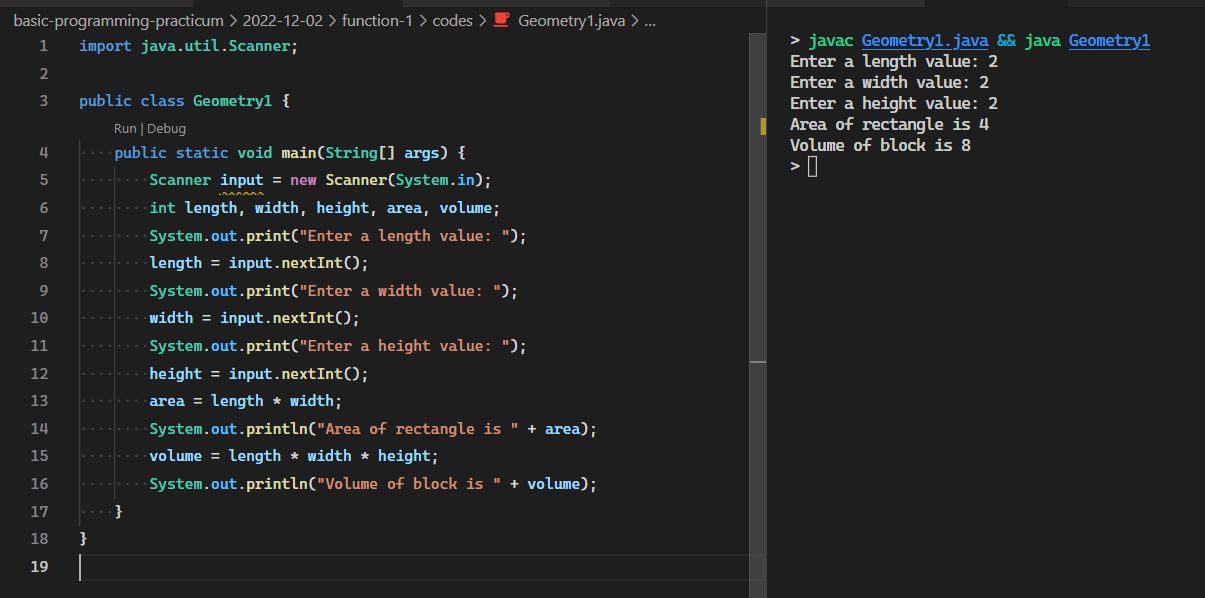
\includegraphics[width=.7\textwidth]{./images/geometry-one.png}
            \caption{Experiment 6 \texttt{Geometry1} code and output}
        \end{figure}

        \begin{figure}[h]
            \centering
            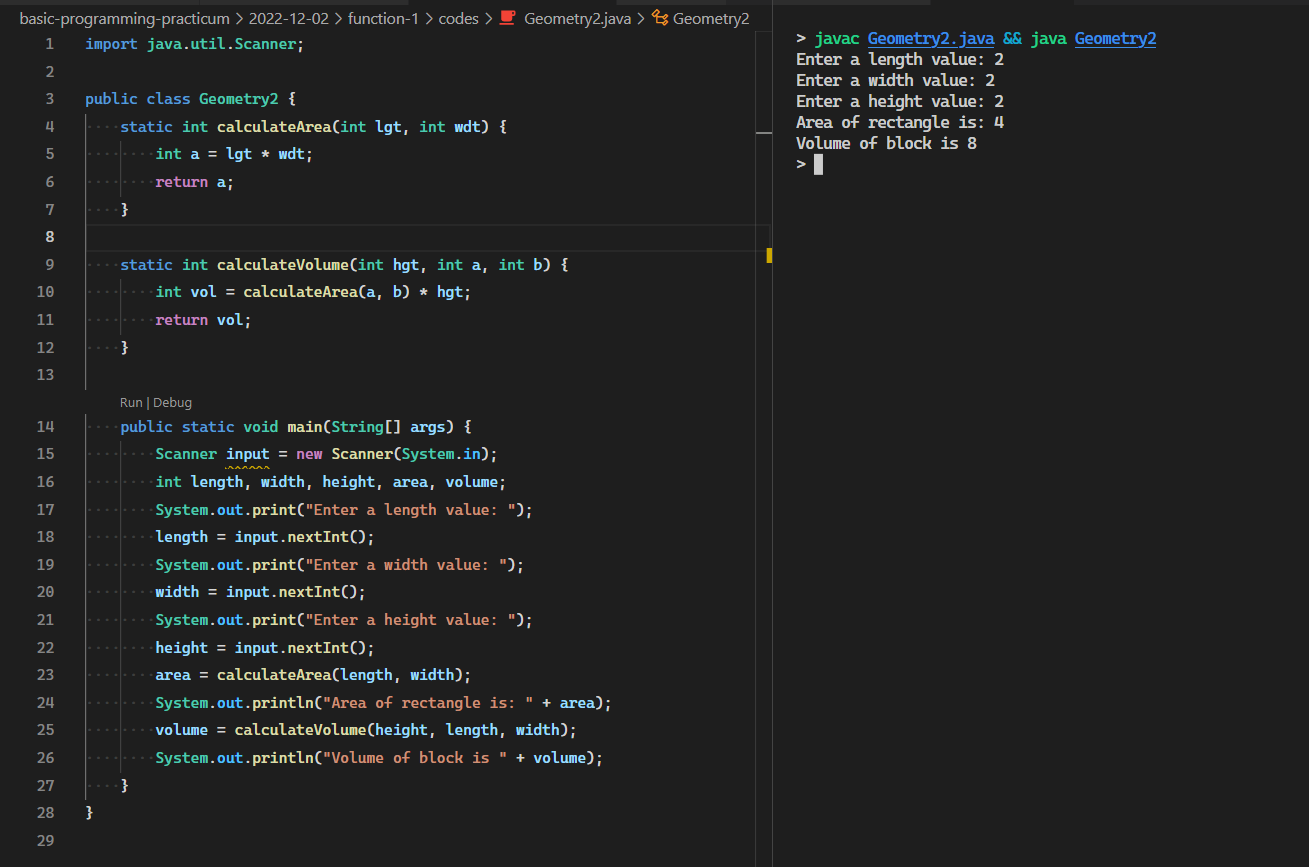
\includegraphics[width=.7\textwidth]{./images/geometry-two.png}
            \caption{Experiment 6 \texttt{Geometry2} code and output}
        \end{figure}
    }
    \pagebreak
    \item {
        Describe the flow of the program for calculating the area of a rectangle and volume of blocks
        in class Geometry2

        \begin{itemize}
            \item The length, width, and height is asked from the user using Scanner
            \item After inputting those values, it calculates the area using the method \\ \texttt{calculateArea} that has been declared before
            \item Inside the \texttt{calculateArea}, the width and height is multiplied
            \item When the area has been calculated, it outputs the value
            \item Next, the volume is calculated using the \texttt{calculateVolume} method that has been declared before
            \item Inside the \texttt{calculateVolume} method, it finds the area using \\ \texttt{calculateArea} method and multiply it with the height
            \item It outputs the volume after it being calculated
        \end{itemize}
    }
\end{enumerate}

\section{Questions!}
\begin{enumerate}
    \item {
        Based on experiment 2 and 3, explain when a function requires a return value!

        A function should return a value when the caller of the function wants a value
        from calling the function.
    }
    \item {
        In Experiment 4, add a function that is used to ensure that the \texttt{value1} and \texttt{value2}
        are at least 0, then call that function in the \texttt{main}!

        \begin{figure}[h]
            \centering
            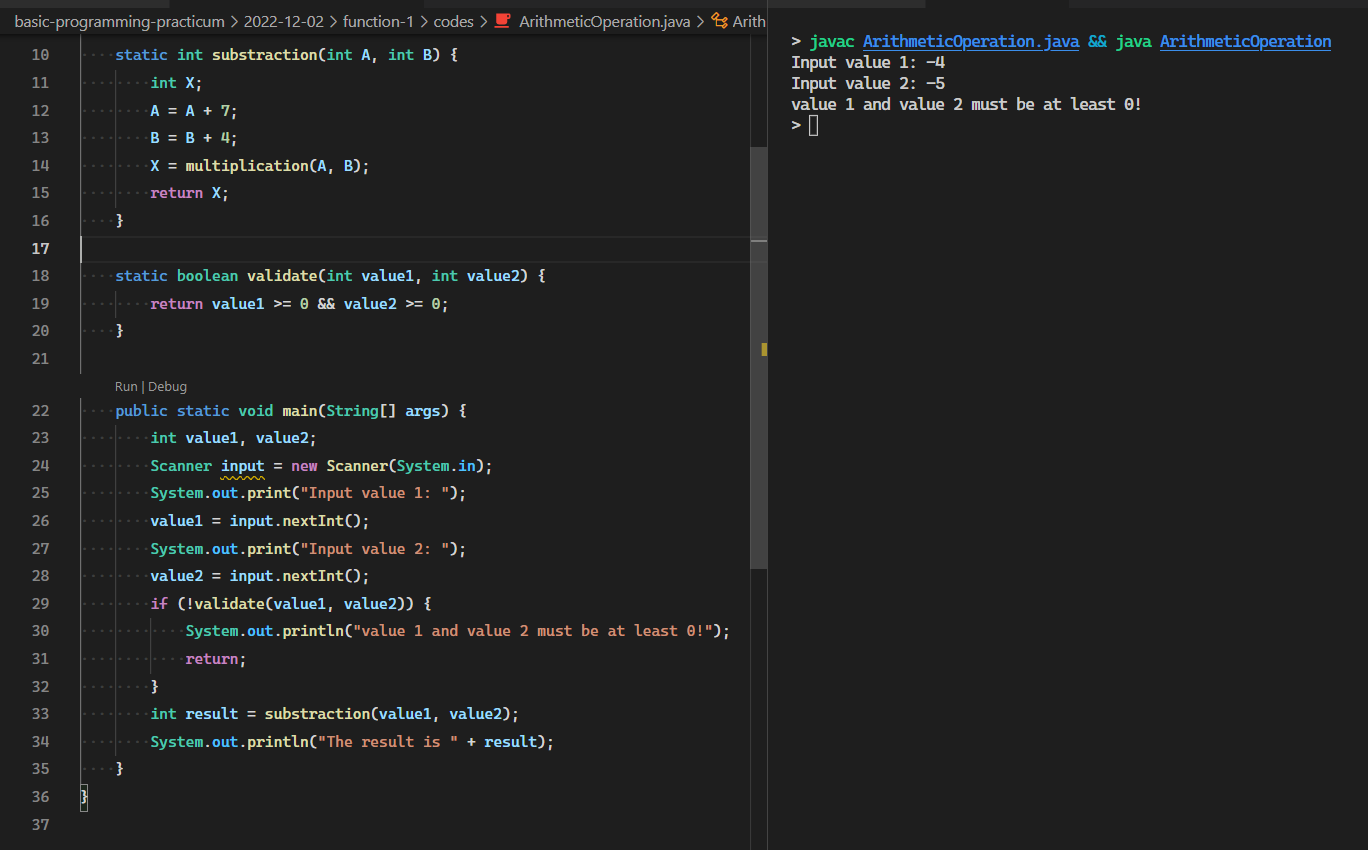
\includegraphics[width=.8\textwidth]{./images/arithmetic-operation-validation.png}
            \caption{Question 2 code and output}
        \end{figure}
    }
    \pagebreak
    \item {
        Explain why the parameter entries in Experiment 5 are written with \texttt{int... a}!

        It's a syntax for \textit{variable arguments} or \textit{varargs} for short. It is used
        so that we can pass in an arbitrary number of arguments into the function and
        the function will collect it as an array that can be used inside the function.
    }
    \item {
        What is the output of the program below, then explain the flow of the program!

        \begin{minted}[autogobble,fontsize=\small]{java}
            public class MyProgram {
                static void printUntil(int i) {
                    for (int j = 1; j <= i; j++) {
                        System.out.print(j);
                    }
                }

                static int total(int num1, int num2) {
                    return num1 + num2;
                }

                static void printTotal(int num1, int num2) {
                    printUntil(total(num1, num2));
                }

                public static void main(String[] args) {
                    int temp = total(1, 1);
                    printTotal(temp, 5);
                }
            }
        \end{minted}

        \begin{figure}[h]
            \centering
            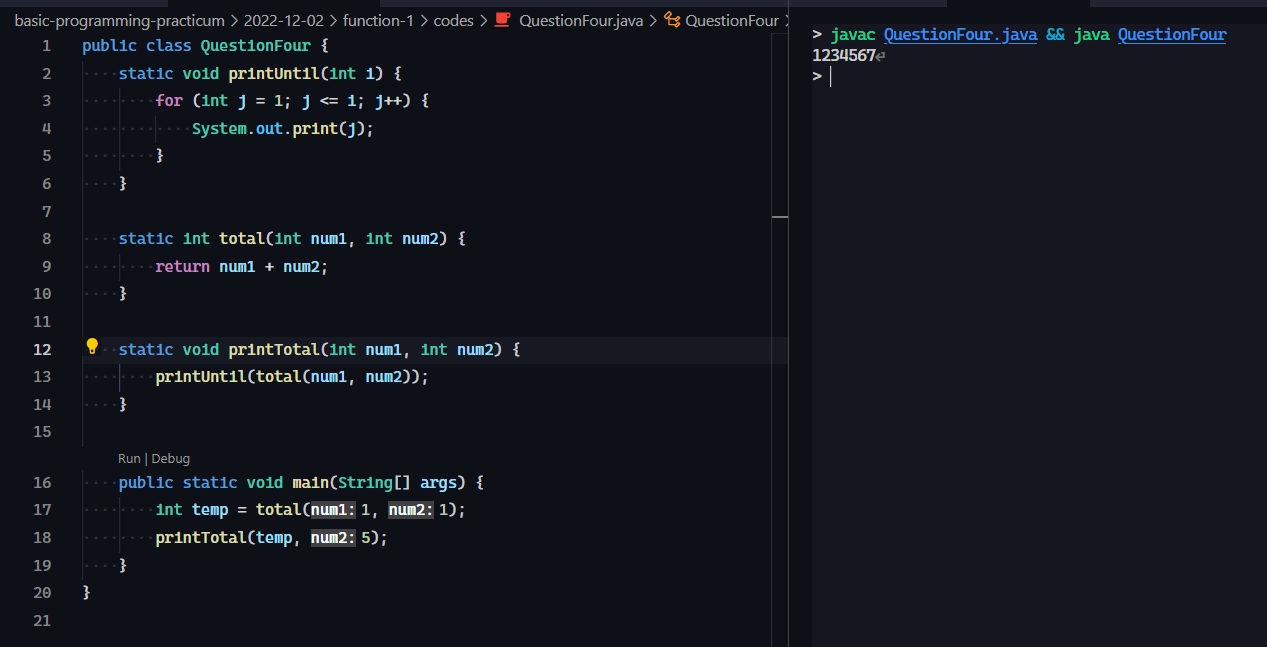
\includegraphics[width=.8\textwidth]{./images/question-four.png}
            \caption{Question 4 code and output}
        \end{figure}

        \begin{itemize}
            \item Starting from main, it will call the \texttt{total} function with an argument of 1 and 1
            \item Inside the \texttt{total} function, it will sum \texttt{num1} and \texttt{num2}
            \item In this case, the return value is an integer of \texttt{2} because $1 + 1 = 2$
            \item After getting the value from \texttt{total}, it calls the \texttt{printTotal} function with an argument of \texttt{temp} and 5
            \item Inside the \texttt{printTotal} function, it will invoke the \texttt{printUntil} functino with an argument of \texttt{total(num1, num2)}
            \item \texttt{total(num1, num2)} will result in 7 because \texttt{num1} will be 2 and \texttt{num2} will be 5
            \item The \texttt{printUntil} function will print the value of \texttt{j} for \texttt{i}-many times, in this case 7 times
        \end{itemize}
    }
\end{enumerate}

\section{Assignment}
\begin{enumerate}
    \item {
        Create a static method called \texttt{Max3(int bil1, int bil2, int bil3)} which takes
        three integer parameters and returns an integer number which is the maximum value among
        the three numbers. Note: You can create other static methods besides \texttt{Max3}.
        After that, call the \texttt{Max3} static method in your \texttt{main} method.

        \begin{figure}[h]
            \centering
            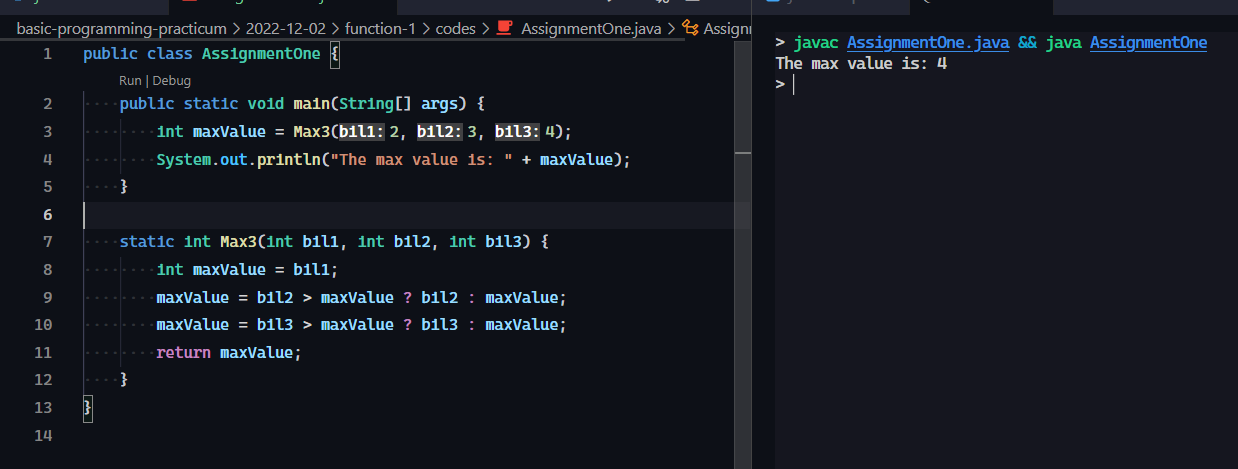
\includegraphics[width=\textwidth]{./images/assignment-one.png}
            \caption{Assignment 1 code and output}
        \end{figure}
    }
    \pagebreak
    \item {
        Create a class called \texttt{Circle} in which there is a function to calculate the circumference
        of a circle and the area of a circle.

        \begin{figure}[h]
            \centering
            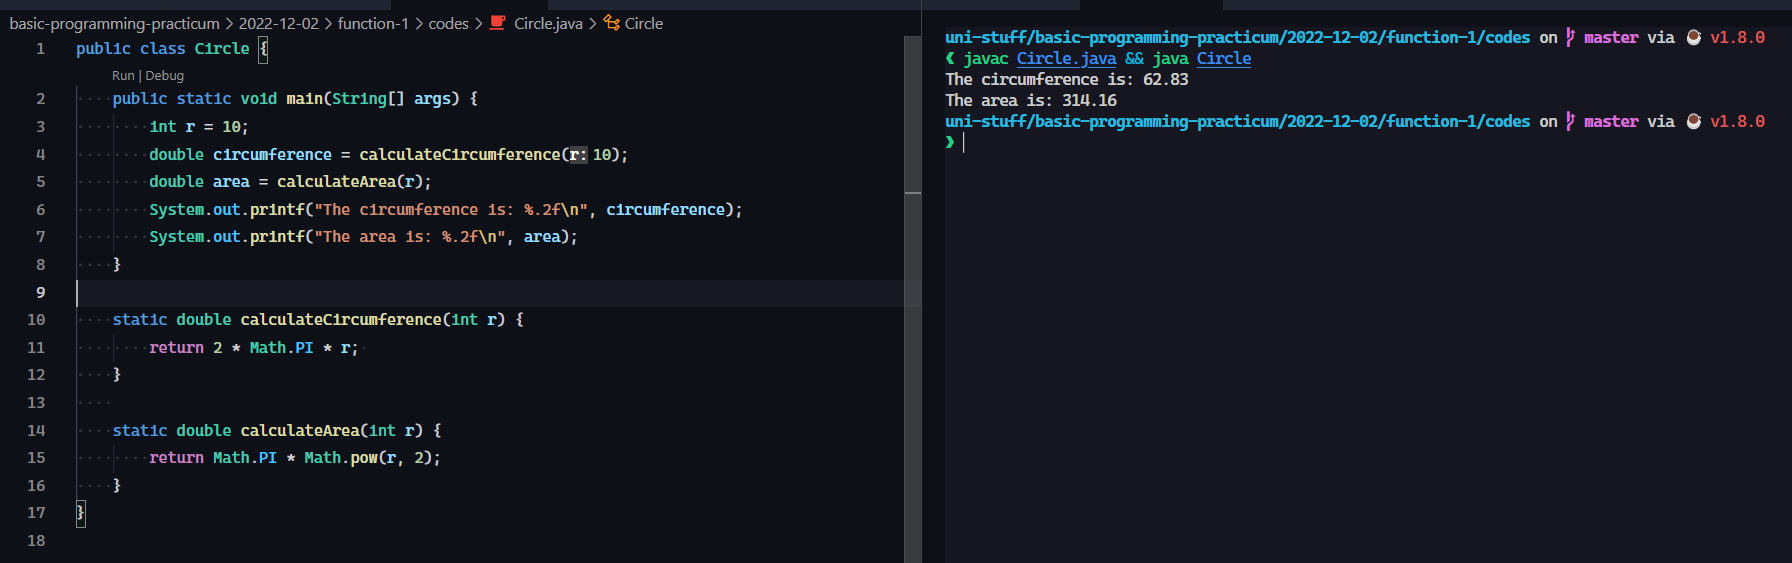
\includegraphics[width=\textwidth]{./images/assignment-two.png}
            \caption{Assignment 2 code and output}
        \end{figure}
    }
    \item {
        Create a program to fill array \texttt{B} with the data type int (10 students' test scores),
        where the input and filling process into the array is carried out in a function. Next, create
        another function to calculate the average value of the array (the average score of students tests).
        Print the average value, with the instructions for printing in the \texttt{main} function.

        \begin{figure}[h]
            \centering
            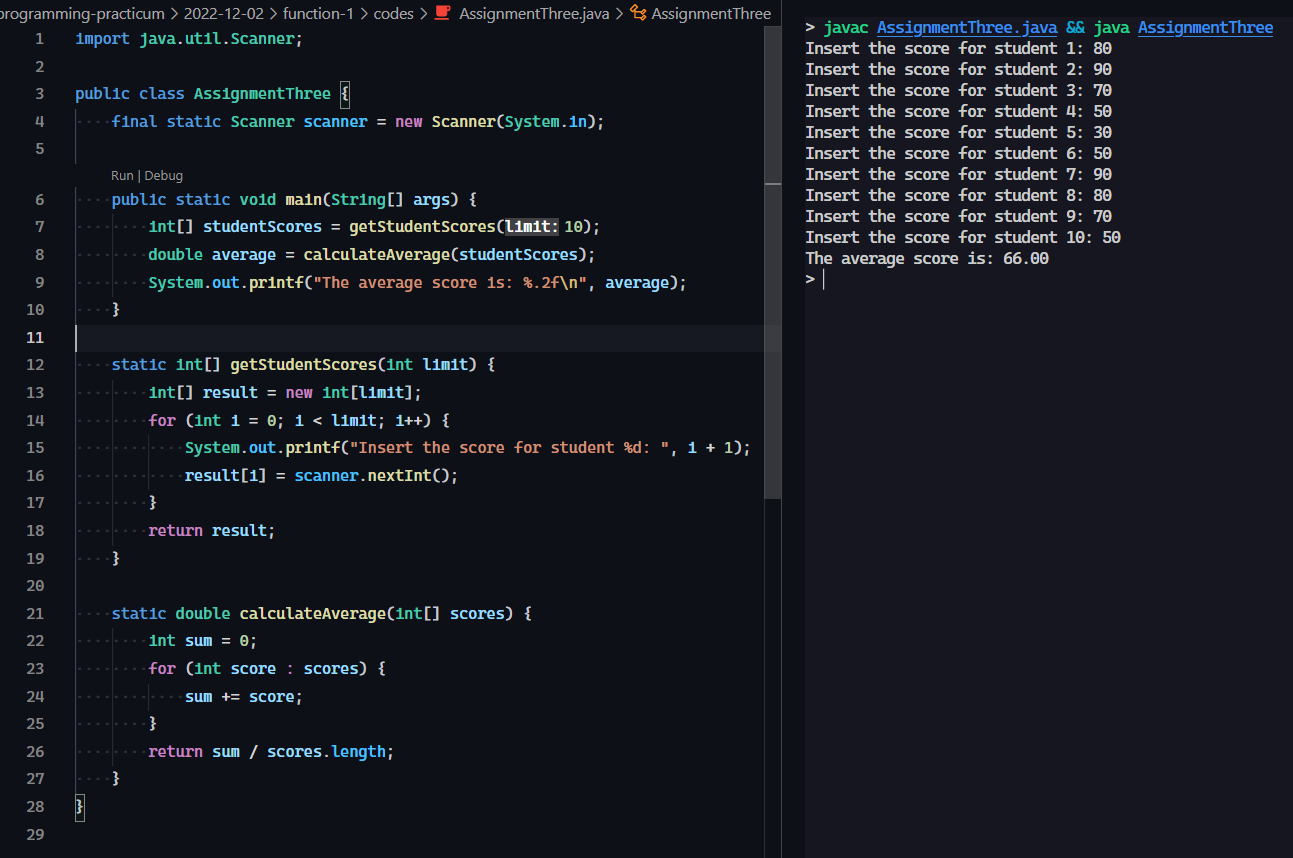
\includegraphics[width=.8\textwidth]{./images/assignment-three.png}
            \caption{Assignment 3 code and output}
        \end{figure}
    }
\end{enumerate}

\end{document}
